% Name: Two-source interference
% Description: Crests spreading from two sources two wavelengths apart, with the lines of constructive interference (m = 0, ±1) and of destructive interference between them.
% Tags: interference, superposition, path difference, wave optics

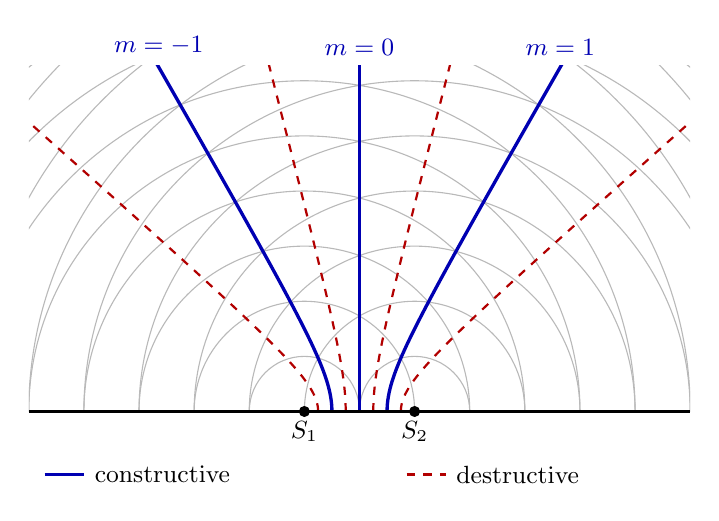
\begin{tikzpicture}[every node/.style={font=\small}]
  % lambda = 0.7, sources at x = +-0.7 (d = 2 lambda); |r1 - r2| = m lambda is the hyperbola with a = m lambda/2, c = 0.7, b = sqrt(c^2 - a^2).
  \begin{scope}
    \clip (-4.2,0) rectangle (4.2,4.4);
    \foreach \r in {0.7,1.4,...,6.3} \draw[gray!55] (-0.7,0) circle (\r) (0.7,0) circle (\r);
    \draw[very thick, blue!70!black] (0,0) -- (0,4.4);
    \foreach \s in {1,-1} {
      \draw[very thick, blue!70!black, domain=0:3, samples=40] plot ({\s*0.35*cosh(\x)}, {0.606*sinh(\x)});
      \draw[thick, dashed, red!70!black, domain=0:3, samples=40] plot ({\s*0.175*cosh(\x)}, {0.678*sinh(\x)});
      \draw[thick, dashed, red!70!black, domain=0:3, samples=40] plot ({\s*0.525*cosh(\x)}, {0.463*sinh(\x)});
    }
  \end{scope}
  \draw[thick] (-4.2,0) -- (4.2,0);
  \fill (-0.7,0) circle (2pt) node[below] {$S_1$} (0.7,0) circle (2pt) node[below] {$S_2$};
  \node[above, blue!70!black] at (0,4.4) {$m = 0$};
  \node[above, blue!70!black] at (2.55,4.4) {$m = 1$};
  \node[above, blue!70!black] at (-2.55,4.4) {$m = -1$};
  \draw[very thick, blue!70!black] (-4,-0.8) -- ++(0.5,0) node[right, black] {constructive};
  \draw[thick, dashed, red!70!black] (0.6,-0.8) -- ++(0.5,0) node[right, black] {destructive};
\end{tikzpicture}
